\subsection{Распределение вычислительной нагрузки с дроблением блоков сетки}

\subsubsection{Дробление блоков}

Одним из важнейших действий управления расчетной блочно-структурированной сеткой при выполнении вычислений на суперкомпьютере является дробление ее блоков \cite{Rybakov2016WithCut}.
Так как при запуске задач на суперкомпьютере постоянно возрастает степень параллельности (используется все больше параллельных процессов обработки блоков сетки), то для сохранения равномерности распределения блоков по вычислительным процессам требуется уметь измельчать блоки.
Блок сетки может быть разделен на два блока по любому из трех направлениий: $I$, $J$, $K$.

Кроме блоков сетка содержит другие объекты, которые требуют корректировки после разделения блока.
Сюда относятся интерфейсы, описывающие касание блоков друг друга.
На границе расчетной области граничные условия задаются с помощью специальных объектов, которые также должны быть разделены в случае пересечения их линией разреза блока.
Также должны быть по необходимости разделены области, описывающие начальные условия.
Каждыий из этих объектов имеет жесткую привязку к блоку, а значит после дробления может возникнуть
необходимость разделения этого объекта.

Граничные условия и области начальных условий обрабатываются наиболее просто и похожим образом.
Рассмотрим, например, граничные условия в двумерном случае (в координатах $IJ$).

\begin{figure}[ht]
	\centering
	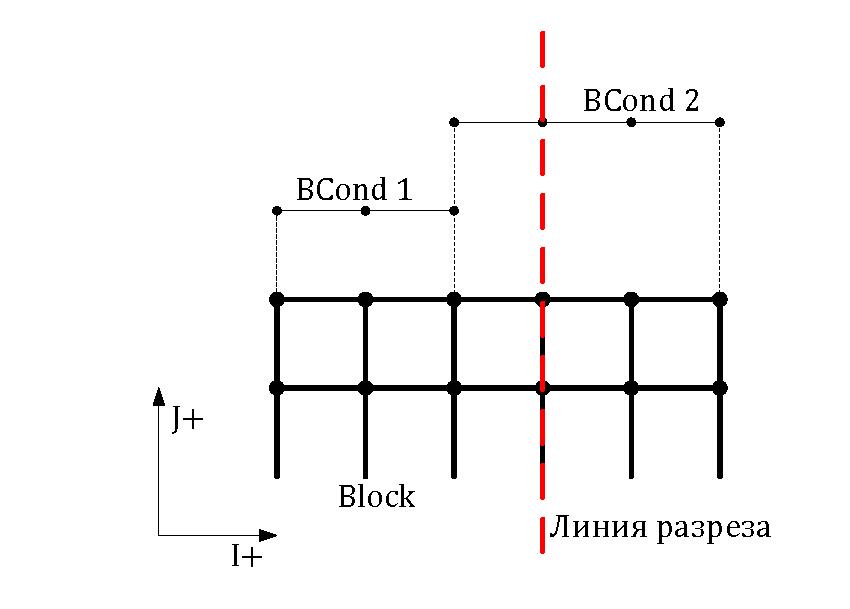
\includegraphics[width=0.6\textwidth]{./pics/text_2_withcut/cut-bcond.pdf}
	\caption{Дробление блока может спровоцировать дробление других объектов сетки.}
	\label{fig:text_2_withcut_cut_bcond}
\end{figure}

Пусть блок Block должен быть разрезан по направлению $I+$ как показано на рис.~\ref{fig:text_2_withcut_cut_bcond}.
Пусть данный блок имеет граничные условия по направлению $J+$.
Тогда возможны два варианта.
Либо линия разреза не пересекает граничное условие, и тогда граничное условие целиком отходит одному из результирующих блоков (BCond 1).
Если же линия разреза проходит через граничное условие, то данное граничное условие также должно быть разделено, и его части отойдут двум результирующим блокам (рис.~\ref{fig:text_2_withcut_cut_bcond2}).

\begin{figure}[ht]
	\centering
	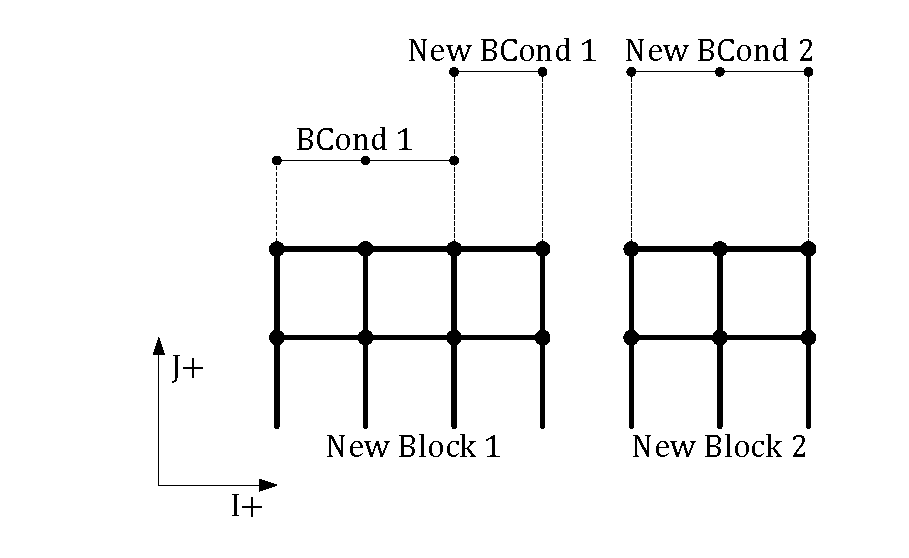
\includegraphics[width=0.6\textwidth]{./pics/text_2_withcut/cut-bcond2.pdf}
	\caption{Разделение граничного условия, спровоцированное дроблением блока.}
	\label{fig:text_2_withcut_cut_bcond2}
\end{figure}

Такая же ситуация может сложиться в отношении областей начальных условий.
В случае дробления интерфейсов могут быть более сложные ситуации дробления.

\subsubsection{Равномерное распределение блоков по вычислительным процессам}

Для равномерного распределения блоков сетки по вычислительным процессам рассмотрим следующую задача разделения множества весов на $m$ различных множеств.

Рассмотрим множество $X$ вещественных чисел $x_i \ge 0$ для $i \in N$, где $N = [1, n]$.
Рассмотрим также множество индексов $j \in M$, где $M = [1, m]$.
Будем говорить, что определено разбиение множества $X$ на $m$ множеств, если введена функция $\gamma(i): N \rightarrow M$.
Множество всех функций разбиения будем обозначать $\Gamma(N, M)$.
Веса результирующих множеств будем определять естественным образом для $j \in M$:
\begin{equation}
	X_j = \sum_{\substack{i \in N \\ \gamma(i) = j}}{x_i}
\end{equation}

Требуется найти такую функцию разбиения $\gamma \in \Gamma(N, M)$, чтобы минимизировать наиболее тяжелое из результирующих множеств: $\min_{\gamma \in \Gamma(N, M)}{\max_{j \in M}{X_j}}$.

Задача может быть расширена на случай распределения вычислительной нагрузки между различными вычислителями суперкомпьютера. При этом формулировка задачи меняется только в части приведения всех узлов к одному показателю с помощью весовых коэффициентов.

Коэффициентом приведения $\kappa(j)$ для $j \in M$ назовем такую положительную функцию $\kappa: M \rightarrow \mathbb{R}_{>0}$, что время выполнения нагрузки $\kappa(j)$ на узле $j$ не зависит от $j$.
Тогда в общем случае задача о равномерном разбиении множества весов на $m$ множеств с коэффициентами приведения $\kappa(j)$ для $j \in M$ формулируется следующим образом.
Требуется найти такую функцию разбиения $\gamma \in \Gamma(N, M)$, чтобы минимизировать наболее тяжелое из результирующих множеств с учетом коэффициентов приведения: $\min_{\gamma \in \Gamma(N, M)}{\max_{j \in M}{\kappa(j) X_j}}$.

Данная задача имеет практическое применение при распределении вычислительной нагрузки между вычислителями гетерогенного суперкомпьютера.

Сформулированная задача является NP-полной, однако ее можно решить приближенно с помощью жадного алгоритма.
В жадном алгоритме будем последовательно обрабатывать все веса, начиная с наибольшего.
Каждый необработанный вес будем относить с наиболее легкому на текущий момент множеству весов.

Приведем без доказательства оценку эффективности работы алгоритма.
Для удобства будем считать, что изначальное множество весов упорядочено по убыванию. 

Определим остаточный член $r_i$ для $i \in N$ по следующей формуле:
\begin{equation}
	r_i = \max{x_i - \frac{1}{m} \sum_{t = i}^{n}{x_t}, 0}
\end{equation}

Тогда можно доказать следующее соотношение
\begin{equation}
	\max_{j \in M}{X_j} - \frac{1}{m} \sum_{j \in M}{X_j} \le \max_{i \in N}{r_i}
\end{equation}

Таким образом, для оценки эффективности описанного жадного алгоритма распределения весов по $m$ множествам достаточно проанализировать ряд остаточных членов, полученный из отсортированного массива распределяемых весов.

Задачу о равномерном распределении весов по результирующим множествам можно применить для равномерного распределения блоков по вычислительным процессам суперкомпьютера в предположении, что все процессы равнозначны (не рассматривается случай гетерогенной системы).
Для этого отметим следующие моменты.
В качестве веса блока нужно взять количество его ячеек.
Так как абсолютно равномерное распределение блоков по вычислительным процессам не всегда возможно, то нужно принять порог максимально допустимого отклонения количества ячеек одного процесса от среднего значения, при достижении которого распределение можно считать успешным.
Экспериментальным путем установлено, что порог максимального отклонения в 10\% является вполне достаточным для достижения эффективного распределения.
Для оценки качества распределения текущего набора весов блоков можно воспользоваться оценками эффективности, приведенными выше.
Если текущее распределение не удовлетворяет допустимому порогу отклонения количества ячеек процесса от среднего значения, то наиболее крупные блоки следует раздробить, после чего повторить оценку распределения.

\subsubsection{Результаты распредедения блоков по процессам}

Предложенные методы равномерного распределения вычислительной нагрузки между узлами суперкомпьютерного кластера были опробованы на суперкомпьютере МВС-10П, находящемся в МСЦ РАН.
Приведем некоторые результаты, которые были получены для двух расчетных сеток.

Первая рассматриваемая сетка, содержит 13 блоков, 80 интерфейсов, 148 граничных условий, 13 областей начальных условий и 5750102 ячейки.
Размер вычислительной окрестности равен 3.

Ниже приведен график, на котором показана статистика общего количества ячеек блоков, а также количества внутренних, граничных и интерфейсных ячеек с учетом кратности.

\begin{figure}[ht]
	\centering
	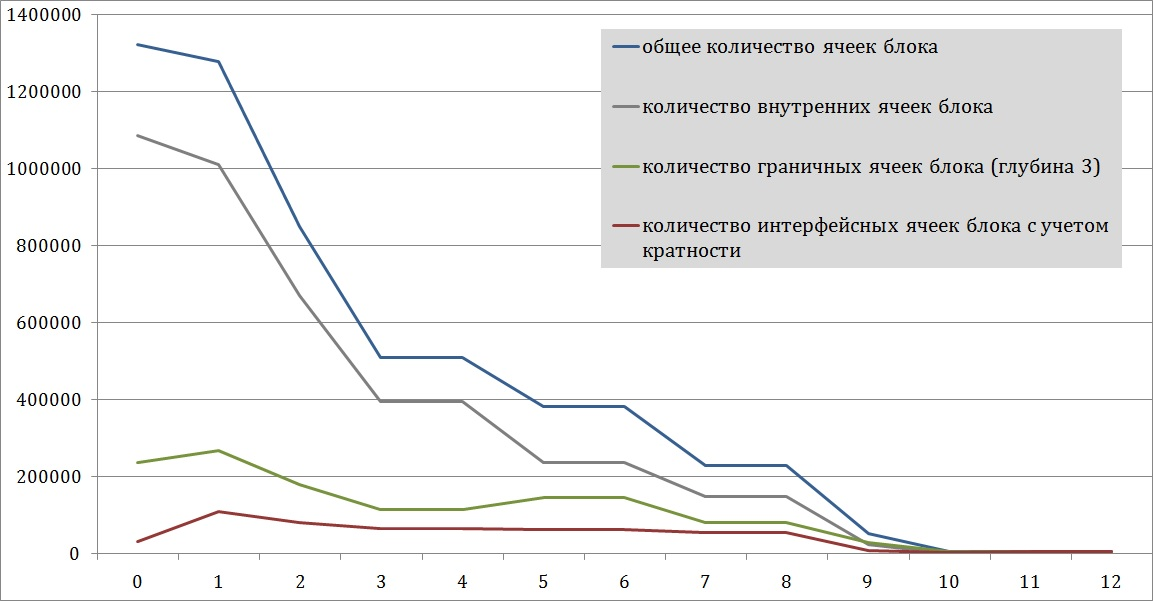
\includegraphics[width=0.6\textwidth]{./pics/text_2_withcut/chart3.jpg}
	\caption{Статистика по количеству ячеек блоков сетки \texttt{vz\_10\_10\_2016}.}
	\label{fig:text_2_withcut_chart3}
\end{figure}

Для этой сетки были проведены вычисления на 128 параллельных процесса.
Приведем статистику распределения блоков по вычислительным процессам для двух различных вариантов: без использования дробления блоков и с использованием дроблений для достижения показателя качества распределения 10\%.

\begin{figure}[ht]
	\centering
	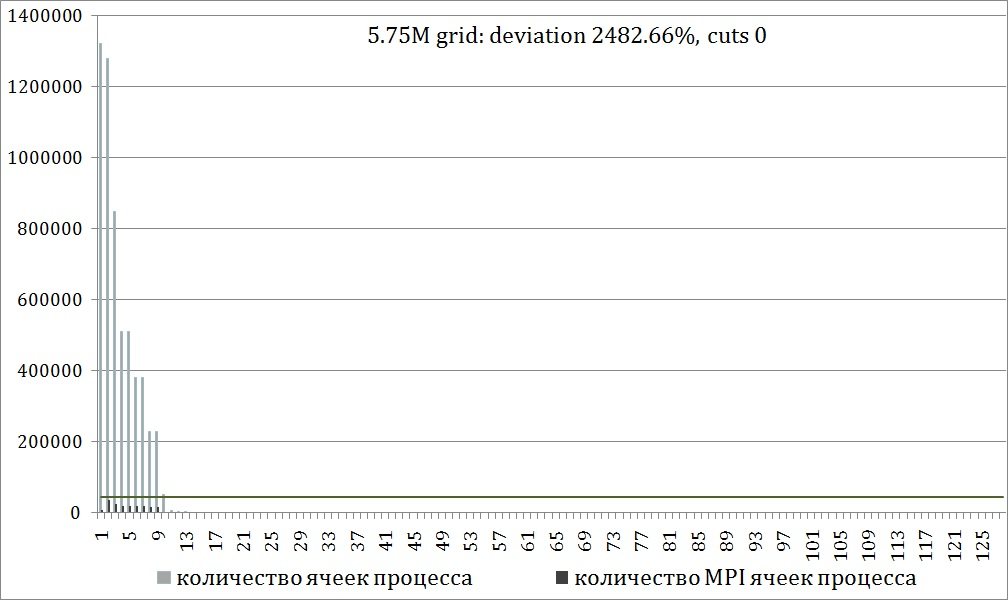
\includegraphics[width=0.6\textwidth]{./pics/text_2_withcut/chart4.jpg}
	\caption{Распределение блоков сетки \texttt{vz\_10\_10\_2016} для 128 процессов без дробления.}
	\label{fig:text_2_withcut_chart4}
\end{figure}

\begin{figure}[ht]
	\centering
	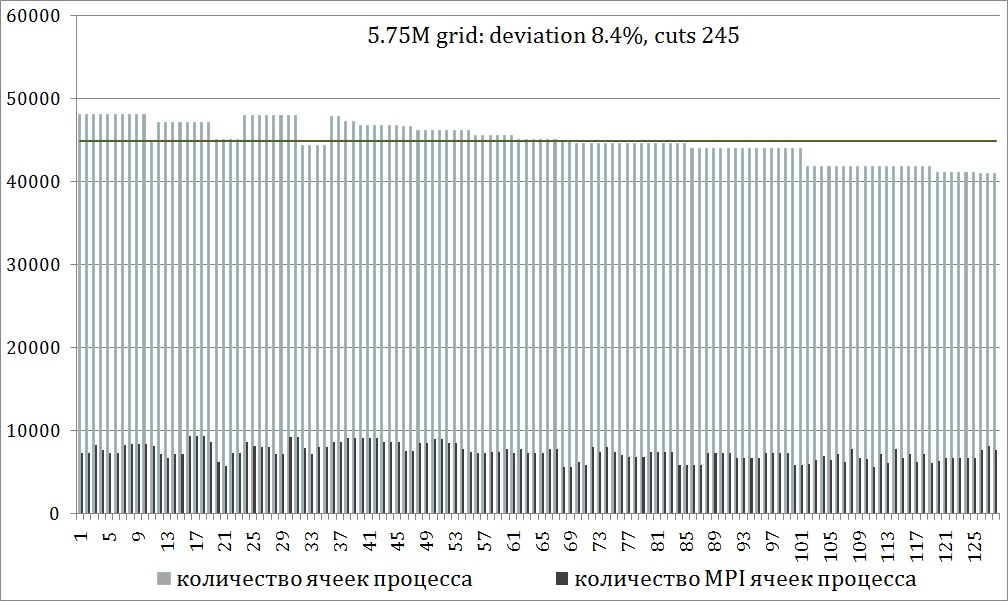
\includegraphics[width=0.6\textwidth]{./pics/text_2_withcut/chart5.jpg}
	\caption{Распределение блоков сетки \texttt{vz\_10\_10\_2016} для 128 процессов с дроблением.}
	\label{fig:text_2_withcut_chart5}
\end{figure}

Аналогичные тестовые запуски производились для сетки, содержащей 300 блоков, 1796 интерфейсов, 1643 граничных условия, 300 областей начальных данных и 94336290 ячейки.
Размер вычислительной окрестности также равен 3.

Ниже приведен график, на котором показана статистика общего количества ячеек блоков, а также количества внутренних, граничных и интерфейсных ячеек с учетом кратности.

\begin{figure}[ht]
	\centering
	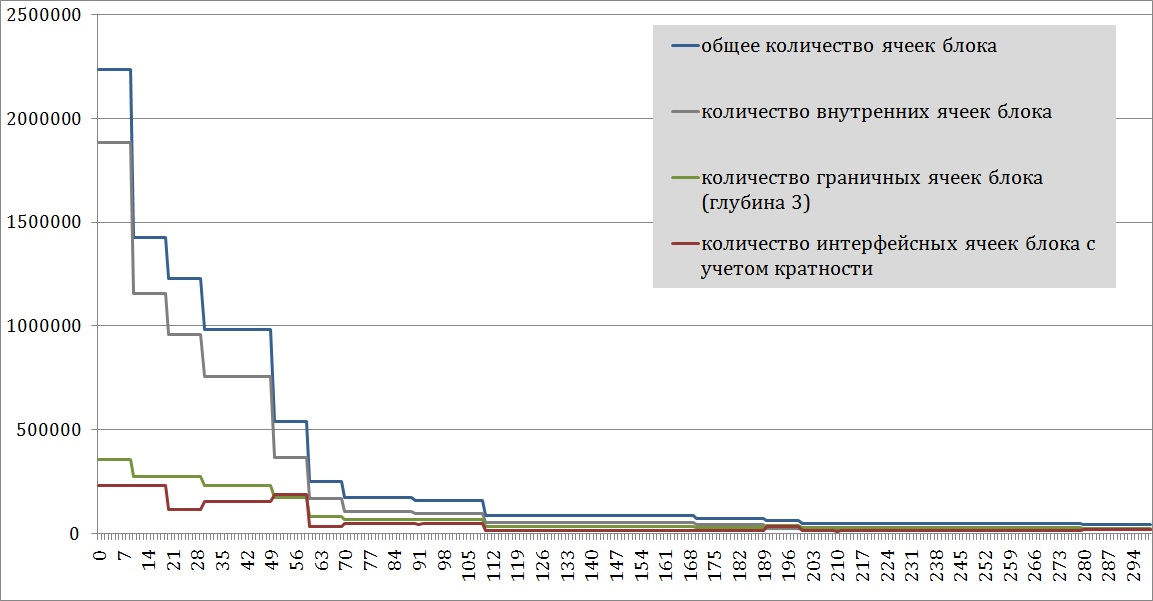
\includegraphics[width=0.6\textwidth]{./pics/text_2_withcut/chart6.jpg}
	\caption{Статистика по количеству ячеек для сетки \texttt{camera\_360\_pill\_nas\_leo\_03\_04}.}
	\label{fig:text_2_withcut_chart6}
\end{figure}

\begin{figure}[ht]
	\centering
	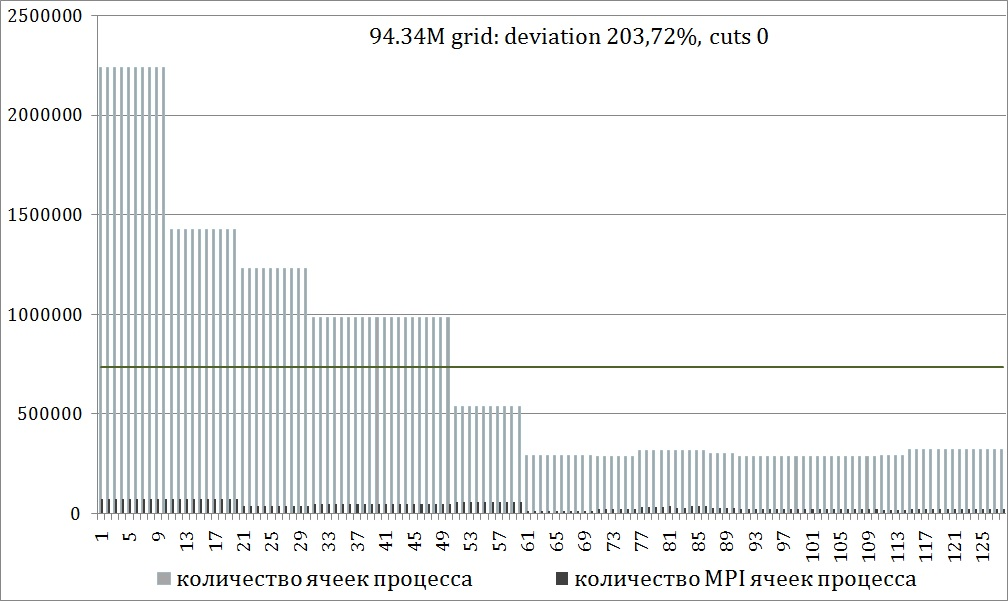
\includegraphics[width=0.6\textwidth]{./pics/text_2_withcut/chart7.jpg}
	\caption{Распределение блоков \texttt{camera\_360\_pill\_nas\_leo\_03\_04}  для 128 проц. без дробления.}
	\label{fig:text_2_withcut_chart7}
\end{figure}

\begin{figure}[ht]
	\centering
	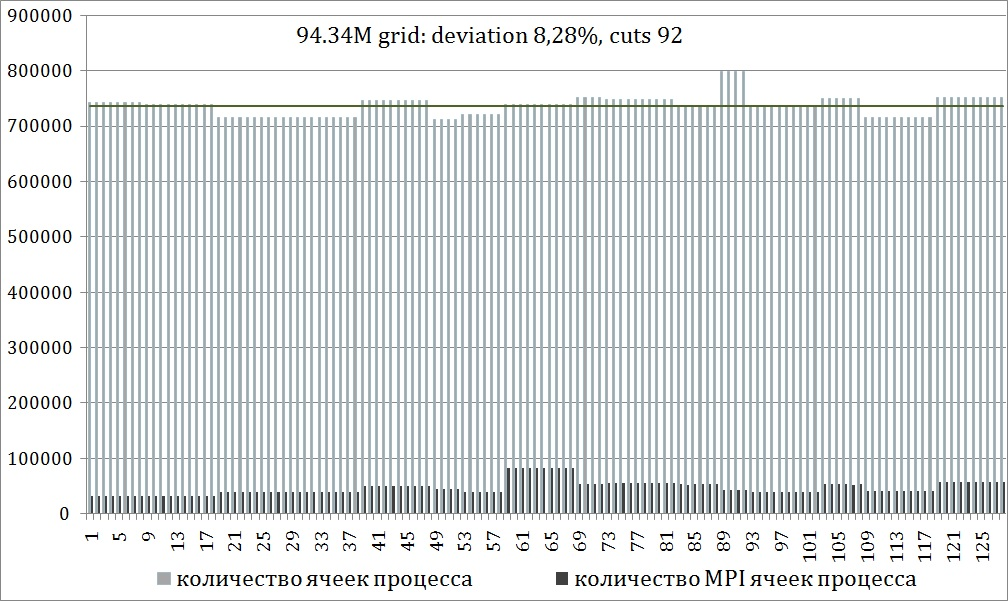
\includegraphics[width=0.6\textwidth]{./pics/text_2_withcut/chart8.jpg}
	\caption{Распределение блоков сетки \texttt{camera\_360\_pill\_nas\_leo\_03\_04} для 128 процессов с дроблением.}
	\label{fig:text_2_withcut_chart8}
\end{figure}

Предложенный механизм равномерного распределения блоков блочно-структурированной сетки между узлами суперкомпьютерного кластера приводит к равномерной загрузке вычислительных ресурсов суперкомпьютерного кластера, что повышает эффективность его использования в расчетах задач газовой динамики. Часто применение такого подхода на большом количестве процессов приводит к кратному ускорению вычислений. Особенно это актуально для сеток содержащих небольшое количество блоков или для сеток, имеющих ярко выраженные крупные блоки.
